% ------------------------------------------------------------------------
% ------------------------------------------------------------------------
% ------------------------------------------------------------------------
%                                Anexo B
% ------------------------------------------------------------------------
% ------------------------------------------------------------------------
% ------------------------------------------------------------------------
% ------------------------------------------------------------------------
\newpage
\anexo{Comparación de la relajación estructural con y sin el parámetro \textsc{u}}\label{anexoB}
% ------------------------------------------------------------------------

En la figura \ref{Fig. rp_ta-nb_e} se presenta la energía estructural en función del grupo de simetría para el material $Sr_{2}(Ta,Nb)O_{3}N$ sin agregar el parámetro \textsc{u} a los cálculos de relajación estructural. La figura \ref{Fig. rp_ta-nb_eU} muestra la comparación entre la energía estructural con y sin el parámetro \textsc{u}$=4eV$.


\begin{figure}[H]
    \centering
    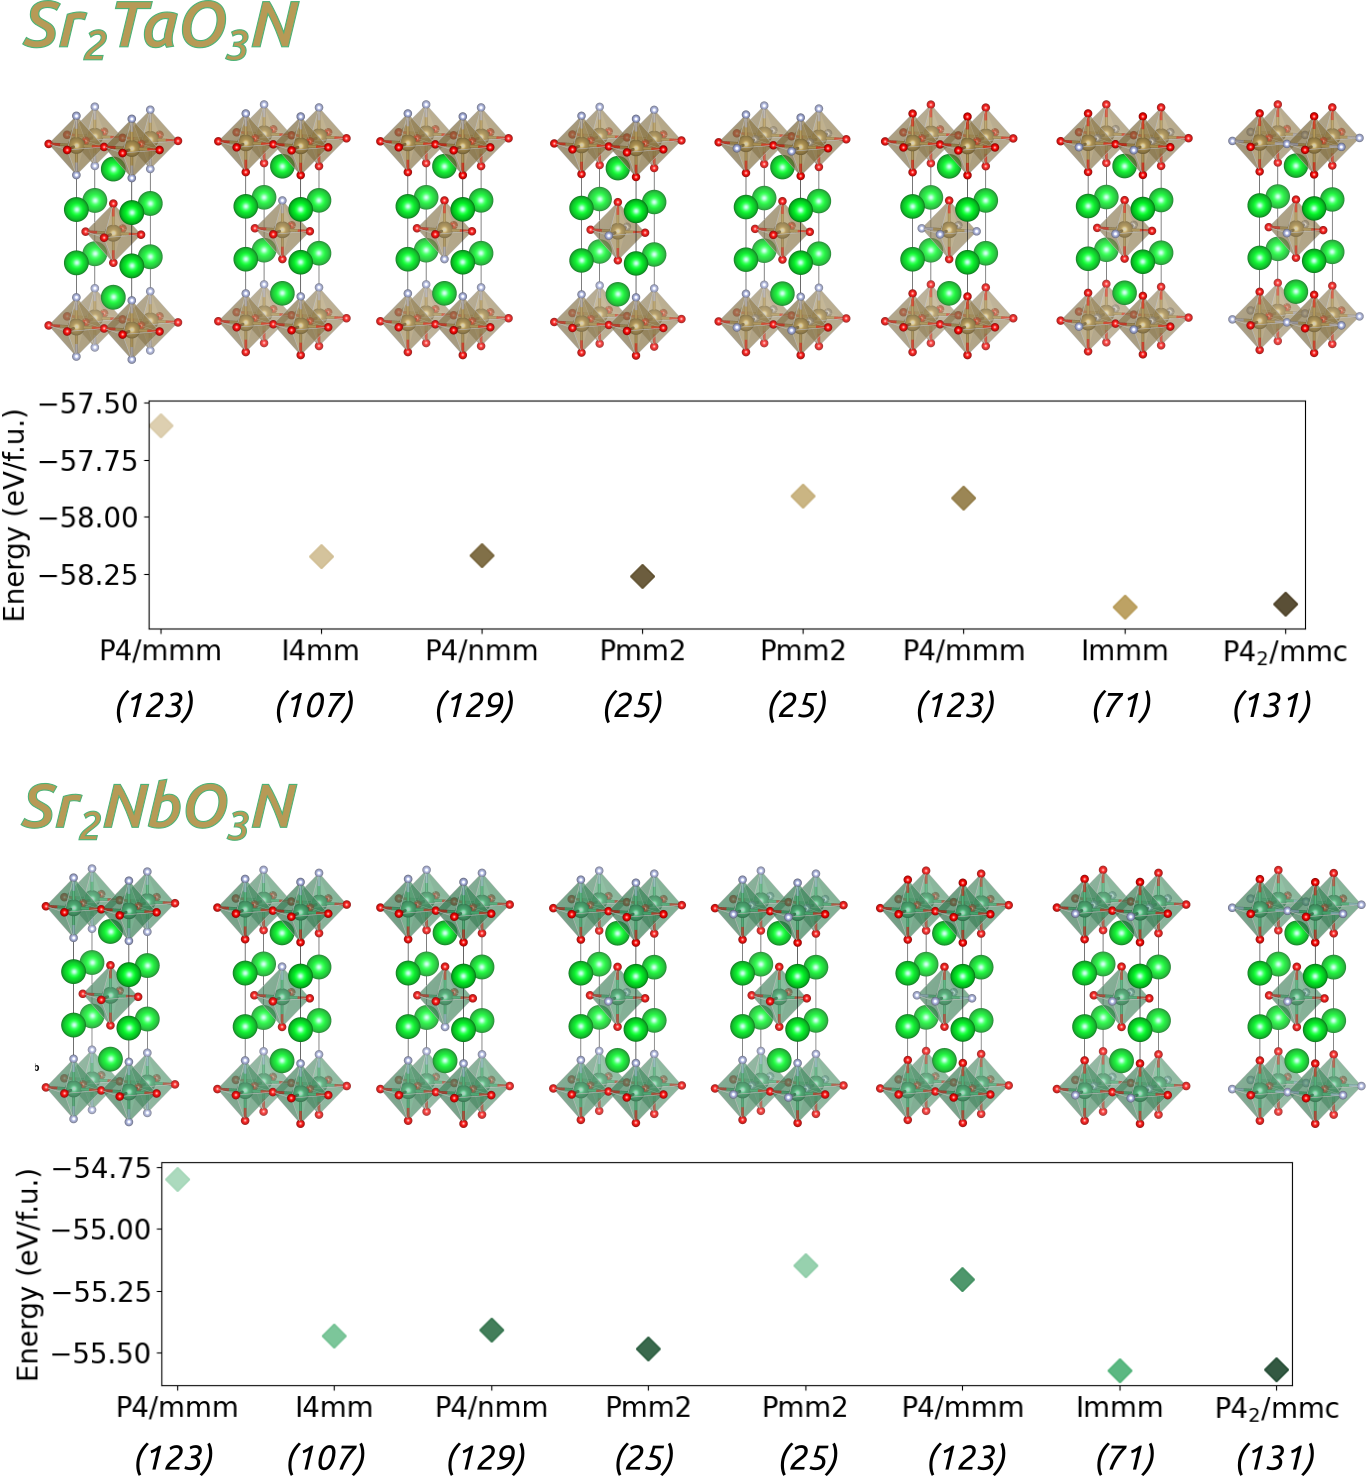
\includegraphics[width=0.9\textwidth]{Figs/rp_ta-nb_e.png}
    \caption{Energía estructural de la concentración $x=1.0$ en función del grupo de simetría espacial para las estructuras Ruddlesden-Popper (arriba) $Sr_{2}TaO_{3}N$ y (abajo) $Sr_{2}NbO_{3}N$.}
    \label{Fig. rp_ta-nb_e}
\end{figure}

Las figuras muestran una diferencia amplia de la energía estructural aportada por \textsc{dft+u} respecto a la energía estructural aportada por \textsc{dft}. Comparando estos resultados calculados con el parámetro \textsc{u} (figura \ref{Fig. rp_ta-nb_energy}) y los resultados sin el parámetro \textsc{u} (figura \ref{Fig. rp_ta-nb_e}): Para el caso de la configuración $Sr_{2}TaO_{3}N$, la energía de cada estructura se ve aumentada en un valor aproximado de $3.25 eV$. Si tomamos un ejemplo para la estructura $Sr_{2}TaO_{3}N$ con grupo de simetría cristalográfico $Immm$(71), la energía sin el parámetro \textsc{u} es de $-58.39eV$, mientras que la energía con el parámetro \textsc{u} es de $-55.15 eV$, es decir existe una diferencia de energía de $-3.24eV$. Para $Sr_{2}NbO_{3}N$, la energía de cada estructura se ve aumentada en un valor aproximado de $3.75 eV$ .Si se hace el mismo análisis para la estructura $Sr_{2}NbO_{3}N$ con grupo de simetría cristalográfico $Immm$(71), la energía sin el parámetro \textsc{u} es de $-55.57 eV$, mientras que la energía con el parámetro \textsc{u} es de $-51.86 eV$, es decir existe una diferencia de energía de $-3.71 eV$. 

Comparando las figuras de energía con y sin \textsc{u} se puede apreciar mas a detalle la diferencia que surge debido a la corrección \textsc{u}. En la figura \ref{Fig. rp_ta-nb_eU} se muestra la comparación de la energía estructural de la fase Ruddlesden-Popper $Sr_{2}(Ta,Nb)O_{4-x}N_{x}$ con y sin el parámetro \textsc{'u'}, tomando en $0.0$ la referencia de la estructura de máxima energía, es decir para las energías calculadas sin el parámetro \textsc{'u'} se toma como referencia la estructura de máxima energía, lo mismo se hace para las energías calculadas con el parámetro \textsc{'u'}.  Ahora quedan barreras de energía reales entre la estructura de mas alta energía y las demás. El hecho de que la energía \textsc{u} afecte mas la configuración con niobio que la configuración con tántalo es debido al tamaño de los átomos. El tántalo es un átomo mas grande, los orbitales están mas lejos, esto hace que entregue los portadores de carga al nitrógeno y al oxigeno mucho mas fácil, pero en el caso de la configuración con niobio, el átomo es mas pequeño, los orbitales están mas cerca del núcleo, esto hace que existan mas problemas de correlación\cite{acgarcia22july}. Los grupos de simetría cristalográficos no cambian respecto a los resultados previos sin el parámetro \textsc{u} debido a que este parámetro  se agrega como una energía en los orbitales y los corrige\cite{acgarcia15july}, mas no afecta las posiciones atómicas.

\begin{figure}[H]
    \centering
    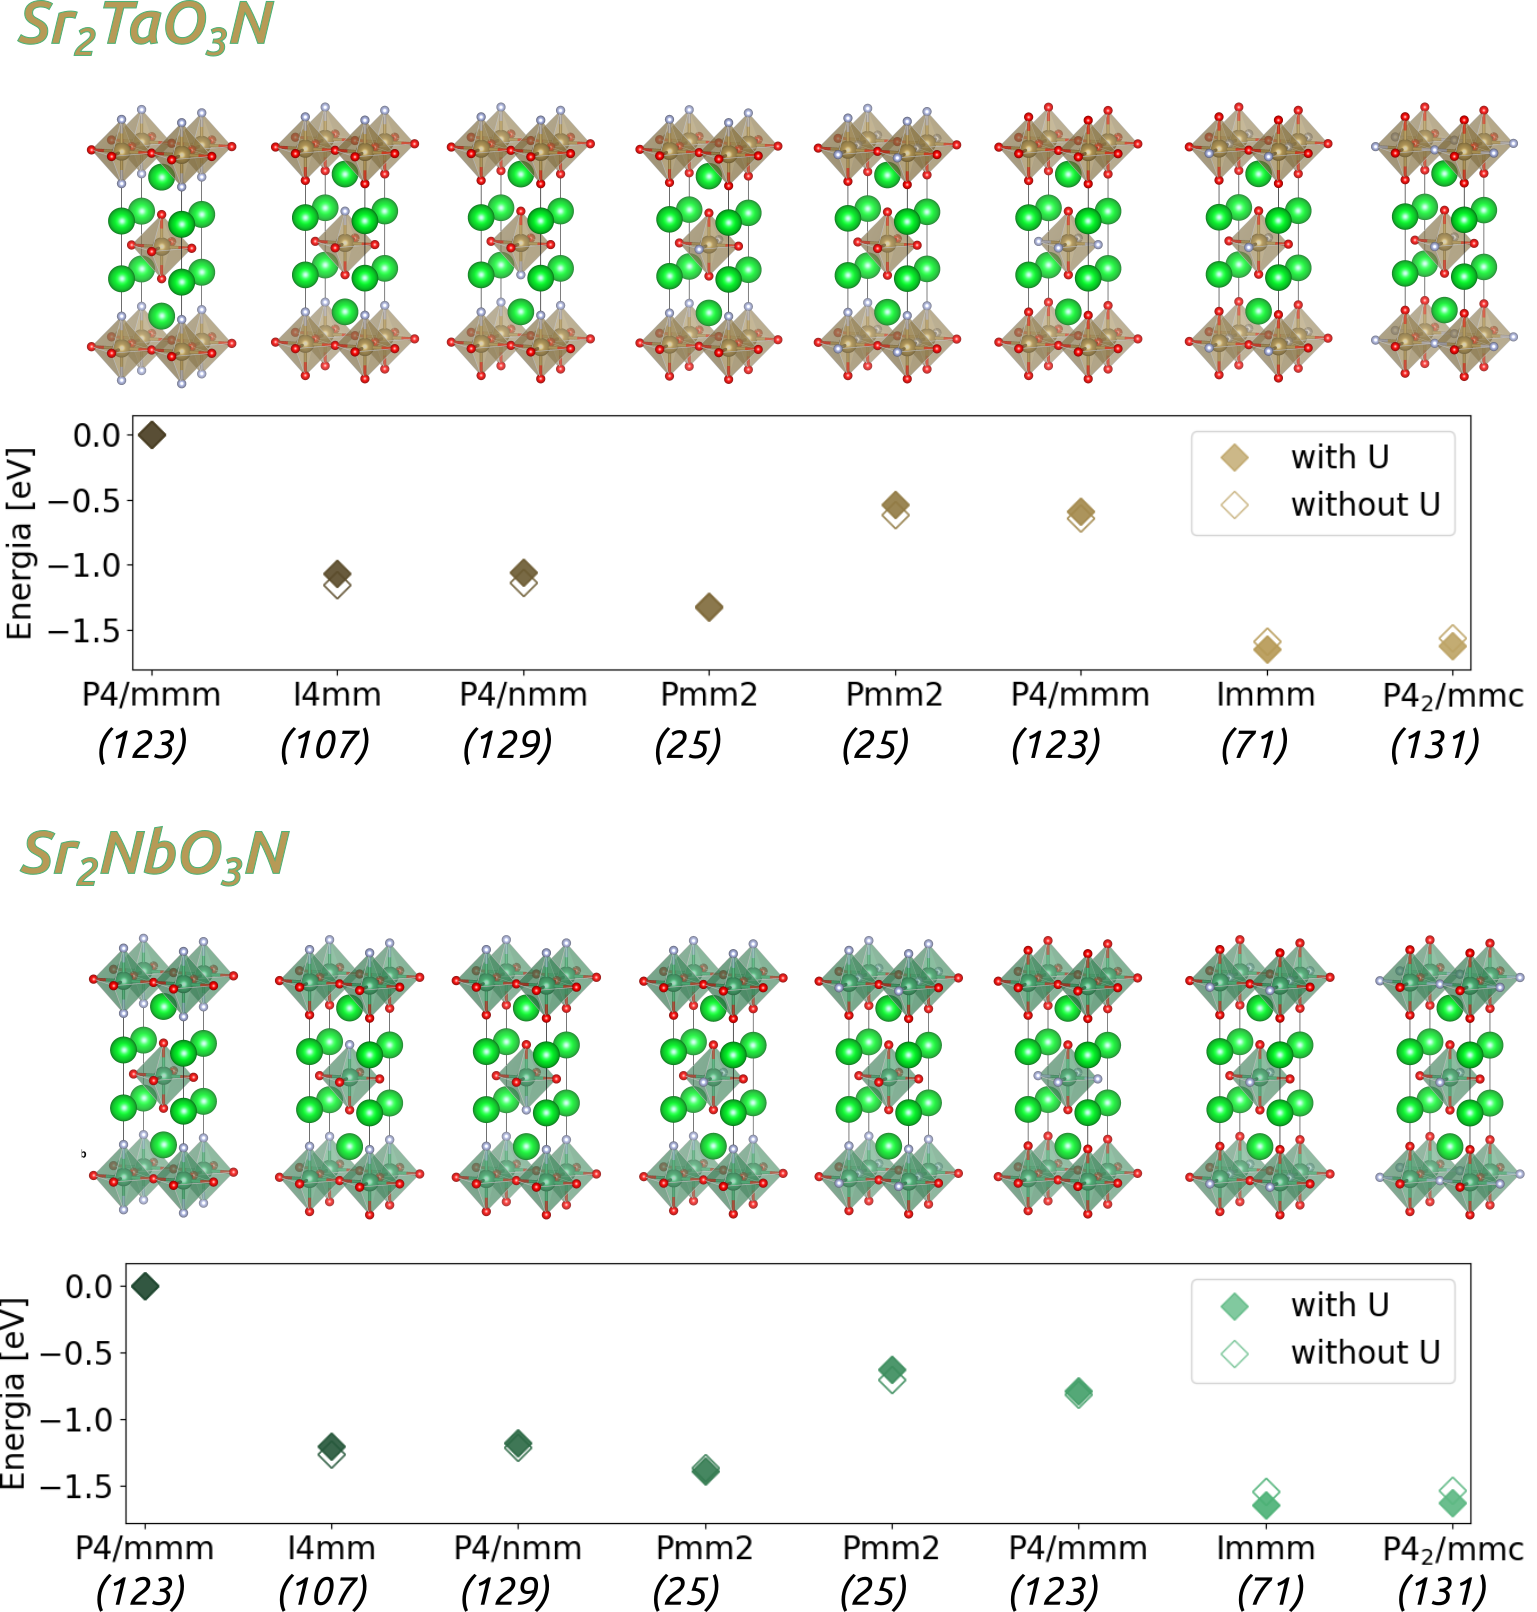
\includegraphics[width=0.9\textwidth]{Figs/rp_ta-nb_eU.png}
    \caption{Energía estructural de la fase Ruddlesden-Popper $Sr_{2}(Ta,Nb)O_{3}N$ en relación a la simetría de grupo espacial a la que corresponde cada estructura.}
    \label{Fig. rp_ta-nb_eU}
\end{figure}







